\documentclass[a4paper,12pt]{article}
\usepackage[T1]{fontenc}
\usepackage[utf8]{inputenc}
\usepackage{lmodern}
\usepackage[french]{babel}
\usepackage[linktocpage]{hyperref}
\usepackage{multicol}
\usepackage{epstopdf}
\usepackage{graphicx}
\usepackage{floatflt}
\usepackage{time}
\hypersetup{
backref=true,
%permet d'ajouter des liens dans...
pagebackref=true,%...les bibliographies
hyperindex=true, %ajoute des liens dans les index.
colorlinks=true, %colorise les liens
breaklinks=true, %permet le retour à la ligne dans les liens trop longs
urlcolor= blue, %couleur des hyperliens
linkcolor= blue, %couleur des liens internes
bookmarks=true, %créé des signets pour Acrobat
bookmarksopen=true,
%si les signets Acrobat sont créés,
%les afficher complètement.
pdftitle={Mon fabuleux livre}, %informations apparaissant dans
pdfauthor={Pejvan BEIGUI},
%dans les informations du document
pdfsubject={Mac OS X}
%sous Acrobat.
}
%TEXTINPUTS=.../texmf-local/tex/latex//:$TEXINPUTS


\begin{document}

\title{Sleipnir, l’octopode fabuleux}
\date{}


\maketitle
\tableofcontents
\begin{center}
{\Large\href{fr.wikipedia.org}{fr.wikipedia.org}}
\end{center}
\smallskip
\begin{abstract}
Dans la mythologie scandinave, Sleipnir est le cheval fabuleux à huit
jambes d’Odin. On présente ici succinctement l’origine de ce mythe et
sa représentation.
\end{abstract}

\section{Introduction}

Sleipnir est, dans la mythologie nordique, un cheval fabuleux à huit jambes capable de se déplacer au-dessus de la mer comme dans les airs, monture habituelle du dieu Odin. Il est mentionné dans l’Edda poétique\footnote{Odin est considéré comme le di}, série de textes compilés au XIIIe siècle à partir de sources plus anciennes, et dans l’Edda en prose, rédigée à la même époque par Snorri Sturluson. Selon ces deux sources, Sleipnir est le fils du dieu Loki et d'un puissant étalon, Svaðilfari. Décrit comme « le meilleur de tous les chevaux » et le plus rapide, il devient la monture d'Odin qui le chevauche jusque dans la région de Hel ; toutefois, le dieu s'en sert surtout pour traverser le pont Bifröst afin de se rendre à la troisième racine d'Yggdrasil, là où se tient le conseil des dieux. L'Edda en prose donne de nombreux détails sur les circonstances de la naissance de Sleipnir et précise, par exemple, qu'il est de couleur grise.

Sleipnir est également mentionné dans une énigme figurant dans une saga légendaire du XIIIe siècle, la Saga de Hervor et du roi Heidrekr, ainsi que dans la Völsunga saga, comme ancêtre du cheval Grani. L'un des livres de la geste des Danois de Saxo Grammaticus au XIIIe siècle contient aussi un épisode qui, selon de nombreux érudits, concernerait ce cheval. Il est généralement admis que Sleipnir fut représenté sur plusieurs pierres historiées de Gotland vers le VIIIe siècle, notamment la pierre de Tjängvide et la pierre d'Ardre VIII.
\section{Ethymologie}
En vieux norrois, le nom de Sleipnir signifie « planeur », ou « glissant »,
et pourrait avoir un sens proche de « celui qui glisse rapidement ».

\section{Mentions dans les anciens textes}
Les Eddas fournissent de nombreux renseignements sur ce cheval, qui
possède pour caractéristiques constantes le fait d’avoir huit jambes, et d’être
décrit comme « le meilleur de tous les chevaux ».
\subsection{Edda poétique}
Sleipnir apparaît dans l’Edda poétique et est mentionné dans les poèmes
Grímnismál, Sigrdrífumál, Baldrs draumar et Hyndluljóð. Dans Grímnismál,
Grimnir (Odin est alors déguisé et dissimule sa véritable identité) raconte à
un jeune garçon nommé Agnar que Sleipnir est le meilleur de tous les chevaux
(« Odin est le plus grand des Ases, Sleipnir le plus grand des chevaux »).
Dans Sigrdrífumál, la valkyrie Sigrdrífa raconte au héros Sigurðr que les runes
devaient êtres coupées « avec les dents de Sleipnir et sur sa sangle striée ».
Dans Baldrs draumar, lorsque les Ases conversent à propos des cauchemars du
dieu Baldr, Odin pose une selle sur le dos de Sleipnir et tous deux partent en
direction des enfers. La section de la Völuspá hin skamma dans le Hyndluljóð
raconte que Loki fit naître Fenrir avec Angrboða et Sleipnir avec Svaðilfari,
enfin un kenning mentionne « un monstre que l’on pensait le plus funeste, et
qui descendait du frère de Býleist », « frère de Býleist » faisant référence à
Loki.


\subsection{Edda en prose}
Dans l’un des livres de l’Edda en prose (Figure 2), Gylfaginning, Sleipnir
est mentionné pour la première fois au chapitre 15 quand Hár raconte que
chaque jour, les Ases chevauchent à travers le pont Bifröst, puis donne la liste
de leurs chevaux. Cette liste commence avec Sleipnir : « Le meilleur d’entre
eux est Sleipnir, il appartient à Odin et a huit jambes ». Au chapitre 41, Hár
cite une strophe qui mentionne Sleipnir dans le Grímnismál.
%\begin{figure}[h] 
 % 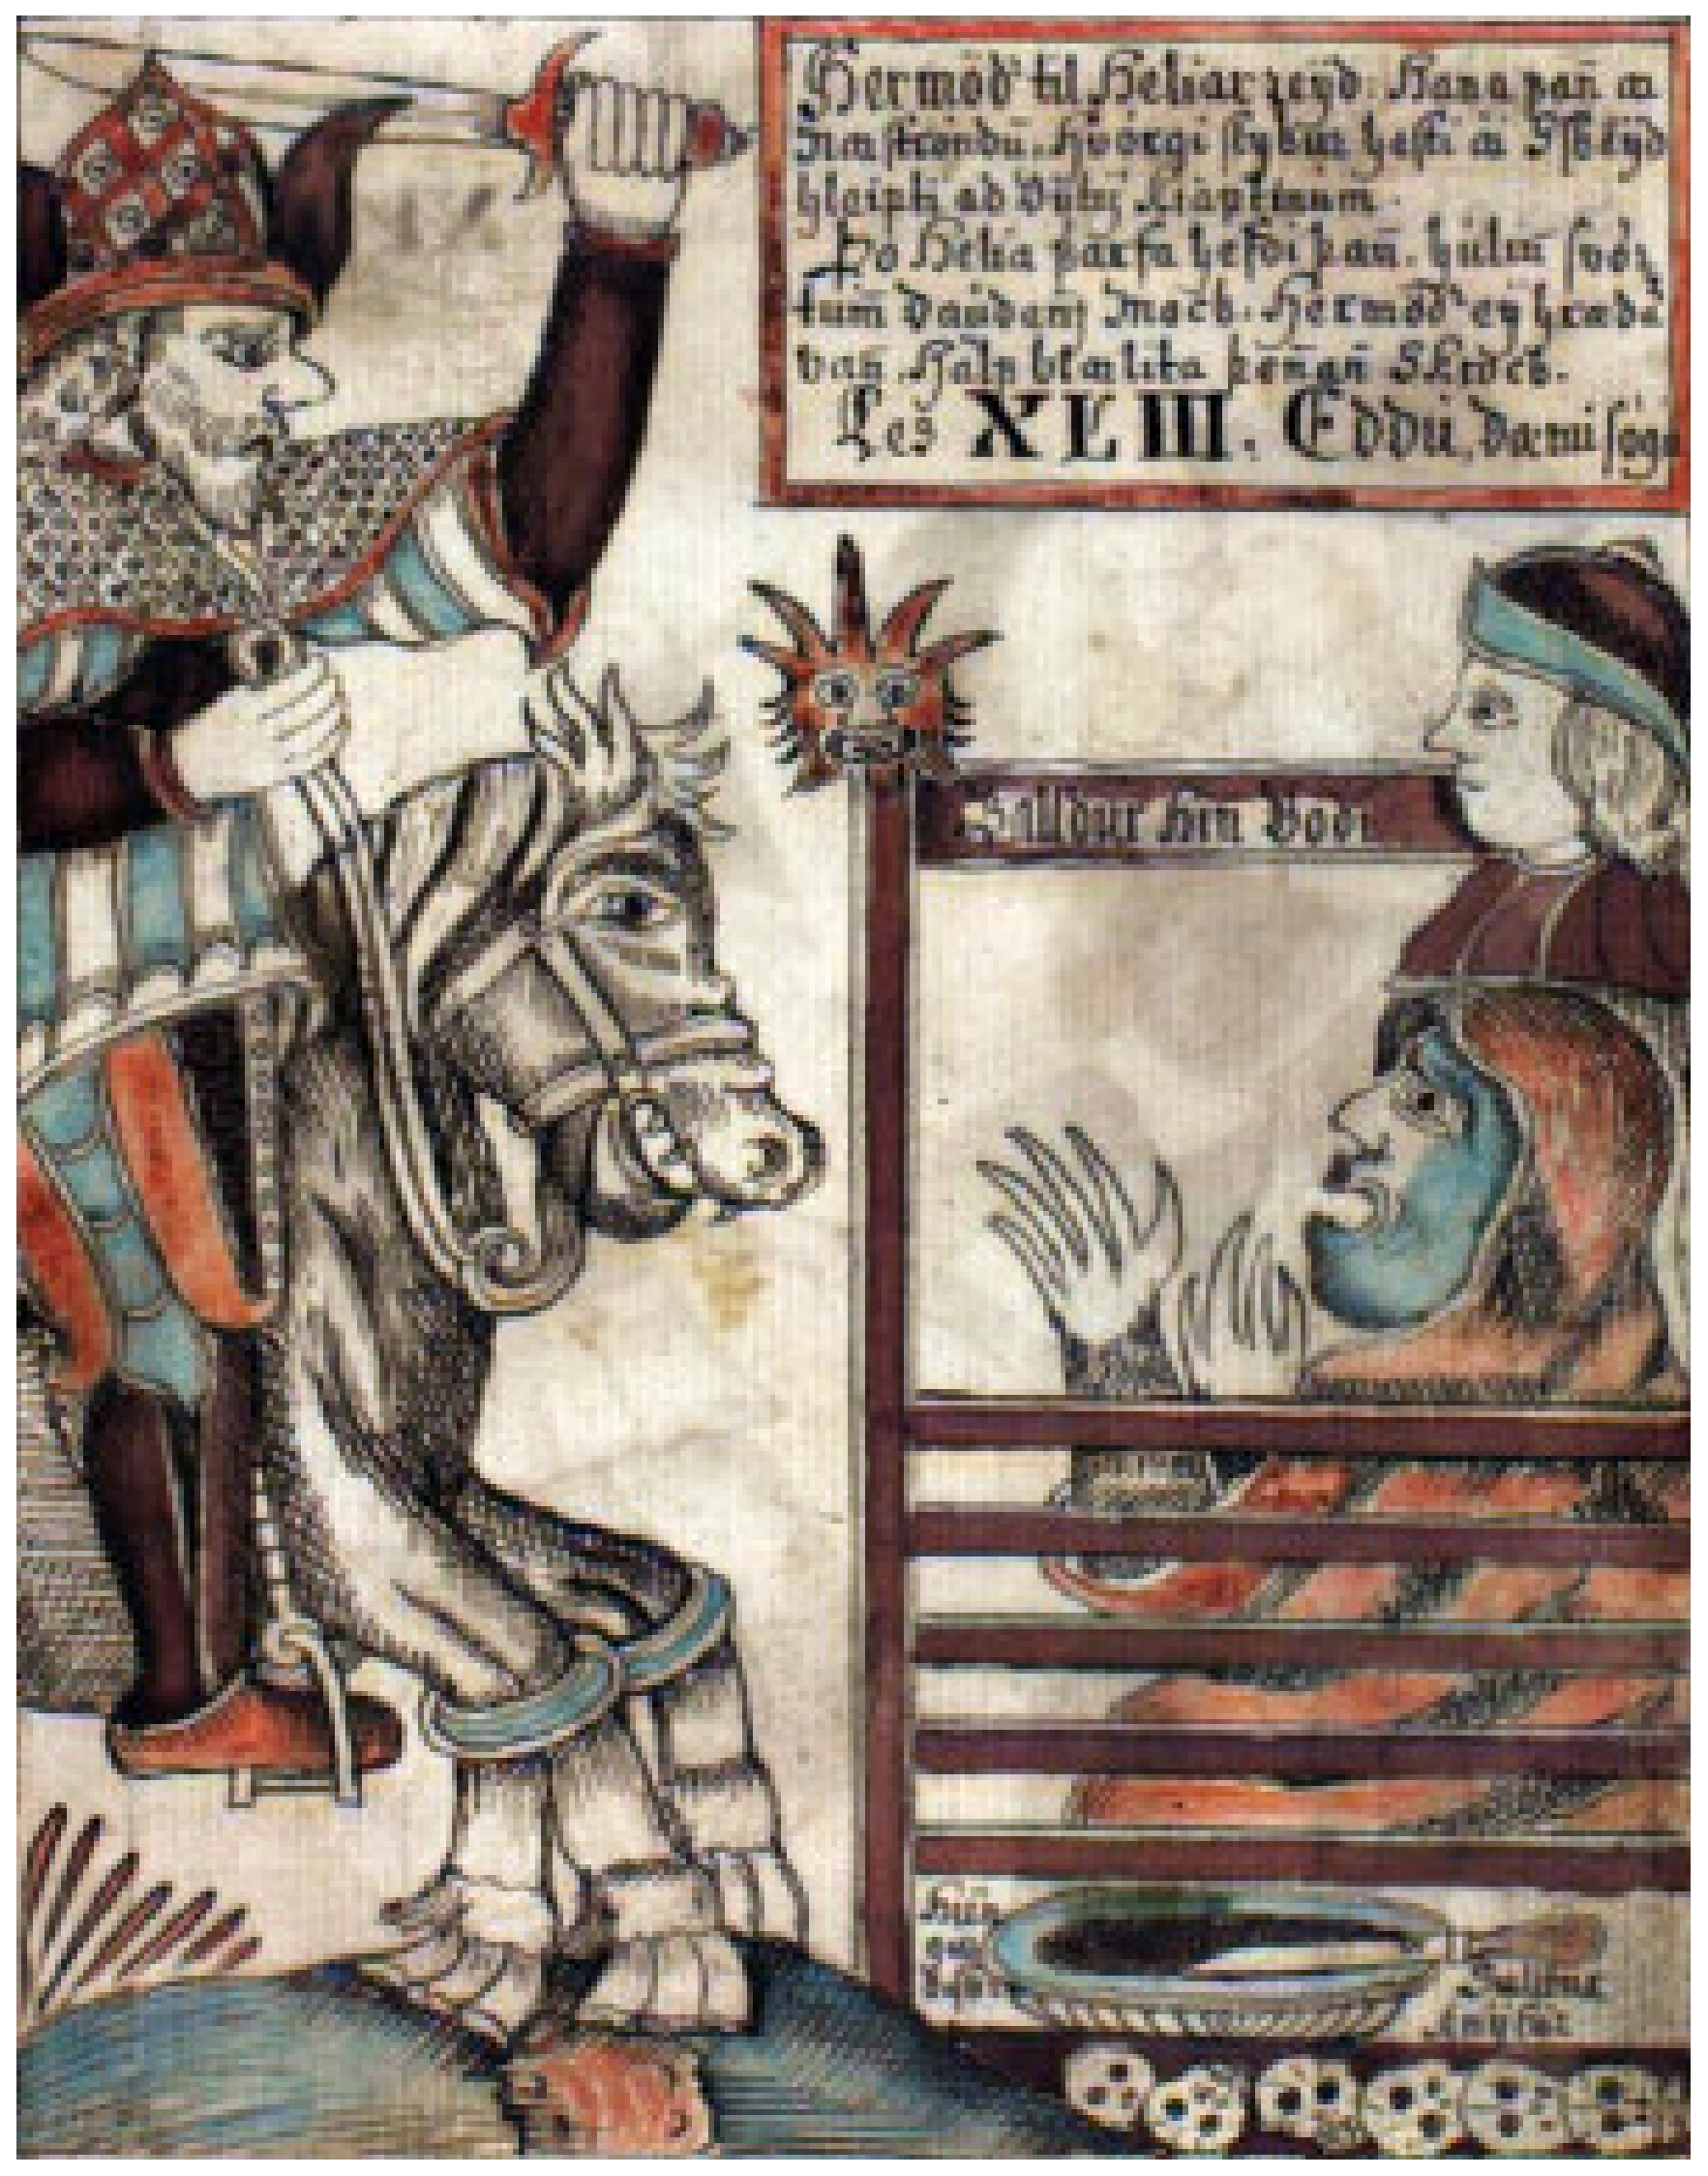
\includegraphics{edda.eps}
%\end{figure} 
\paragraph{Naissance de Sleipnir}
Au chapitre 42, les origines de Sleipnir sont décrites avec précision. Gan-
gleri (mentionné plus tôt dans le livre comme étant le roi Gylfi déguisé)
demande à Hár d’où vient le cheval Sleipnir et ce qu’il peut lui en apprendre.
Hár est surpris par le manque de savoir de Gangleri à propos des origines de
Sleipnir, et raconte l’histoire comme suit : au début, à l’arrivée des dieux,
lorsque ceux-ci eurent établit Midgard et construit le Valhalla, ils reçurent
la visite d’un bâtisseur inconnu qui leur proposa de construire une forteresse
divine imprenable qui les mettrait à l’abri de toutes les invasions en trois
saisons. En échange de ce service, l’étranger demandait le Soleil, la Lune et
Freya. Après quelques débats, les dieux lui donnèrent leur accord s’il s’exé-
cutait en un semestre seulement et sans l’aide de personne. Le bâtisseur
n’eut qu’une requête : il demanda l’autorisation d’utiliser son cheval Svaðil-
fari, et cela lui fut accordé, grâce à l’influence de Loki. À la grande surprise
des dieux, l’étalon Svaðilfari effectuait un travail colossal, et transportait
d’énormes rochers. Avec l’aide de son cheval, le bâtisseur avançait très rapi-
dement, si bien que trois jours avant la date imposée, il ne lui restait plus
qu’à construire la porte. Les dieux, mécontents, conclurent que Loki était la
cause de sa réussite et l’obligèrent à trouver un moyen d’arrêter l’homme.
Ils promirent à ce dernier les plus horribles tourments s’il ne parvenait pas
à trouver un moyen d’empêcher le bâtisseur de terminer son ouvrage dans
les temps et ainsi d’emporter le paiement, et s’apprêtaient à le châtier quand
Loki, effrayé, leur promit de trouver un stratagème. Cette nuit-là, le bâtis-
seur partait chercher les dernières pierres avec son étalon Svaðilfari quand,
au détour d’un bois, il rencontra une jument. La jument hennit en direction
de Svaðilfari et celui-ci, « réalisant quel genre de cheval il était », devint
frénétique, se mit à hennir, déchira ses harnais et se dirigea vers la jument.
Celle-ci courut dans tout le bois, Svaðilfari derrière elle, le bâtisseur tentant
de les rattraper. Les deux chevaux coururent ainsi toute la nuit et les travaux
de construction ne purent avancer d’un pouce pendant les trois nuits qui res-
taient. L’homme, furieux, se transforma en géant car c’était sa vraie nature,
et lorsque les dieux s’en rendirent compte, ils firent fi de leurs serments an-
térieurs et appelèrent Thor. Celui-ci se débarrassa du géant rapidement en
l’assommant avec son marteau Mjöllnir. Toutefois, Loki avait été « fécondé
» par l’étalon du géant, et il donna naissance à un poulain octopode gris
nommé Sleipnir, « le meilleur cheval parmi les dieux et les hommes », qui
devint plus tard la monture d’Odin.

\end{document}
